% Chapter Template

\chapter{Introduction} % Main chapter title

\label{Chapter1} % Change X to a consecutive number; for referencing this chapter elsewhere, use \ref{ChapterX}

\lhead{Chapter X. \emph{Introduction}} % Change X to a consecutive number; this is for the header on each page - perhaps a shortened title

%----------------------------------------------------------------------------------------
%	SECTION 1
%----------------------------------------------------------------------------------------
\section{Electroencephalogram}
An electroencephalogram (EEG) used in evaluation of the brain neuron's electrical activity  . Brain cells uses electrical impulses to communicate to each othe.

An EEG measures electric field fluctuation induced by the  number of electron fluctuation during the neuron communication.The change in the voltage at any reason of brain shows the activity of that region of brain.The measured voltage has to amplified as the is too small in value.The electrodes has been used to measure the voltage,also called channels.In the Figure \ref{fig:eeg},you can see the electrodes are mounted on human brain.
 \begin{figure}
     \centering
     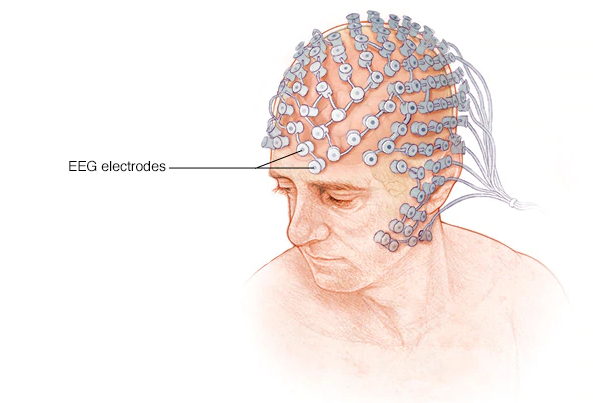
\includegraphics[width=15cm]{Pictures/eeg_1.png}
     \caption{An Image of EEG, showing electrodes \cite{eeg} }
     \label{fig:eeg}
 \end{figure}
\section{Mind Wandering (MW)}
Mind Wandering (MW) is the self-generated thoughts drifting our mind away from the current task. It is a psychological phenomenon that is diverting our attention from a task. MW usually happens while driving \cite{baldwin2017detecting}, reading and other activities where there is less attention. It is a temporary state and is a common trait that people share where they do not remember what was going on in their surroundings since their minds were decoupled. MW can both be intentional and unintentional \cite{seli2017intentionality}. While MW is a common phenomenon, it relates to various psychological problems too.

MW covers about 30-50\% of the waking time which is known to be initiated from the transitions between outwardly steered and self-generated thoughts .EEG is a well-accepted tool in detection of MW to identify artifacts from multi-channel EEG data . It has a few limitations in measuring circumstance, and a passable amount of information is expected. In un-investigated conditions the EEG indicator can divulge the nature of MW.As MW tends to occupy half of our waking time it plays a crucial role in our everyday life. Indeed there are benefits to MW . MW is an essential measure of our self-identity and has also been knotted to creative problem-solving . It results in helping us make plans about the future. MW enhanced human’s creativity above and beyond the positive effects of their reading ability or fluid intelligence, the general ability to solve problems or puzzles . Admittedly, it was found that happiness of a person who is in MW decreases suggesting that a negative mood might be a consequence  of a wandering mind. Besides, it is a menace to transportation safety, resulting in substantial number of crashes and fatalities . Taken together whether MW is good or bad depends on when we mind wander and what we wander about .

Furthermore, reviewing the prior research under this field, a good sum of work has been dedicated in detection of MW. There are numerous existing research works employed to extract various features such as EEG variables and non-linear regression , oculometric features \cite{grandchamp2014oculometric}, incubation paradigm to assess performance , oscillatory activity of the entire brain , spontaneously adopted problem solving approaches using self-reports , kernel size and stride , EEG markers used as features for the classifier  spatial patterns to discover scalp topologies 

\section{Aims And Objectives}

In this project, we explored basic machine learning techniques to predict the mind wandering using EEG signals.In order to achieve a higher accuracy, classification of different combinations of features were done.Random forest classifier gave a higher accuracy than any other ML classifier so applying different classification methods aided our precision level. The main factor in our paper is that we have worked with EEG signals solely to detect MW and has also achieved a promising result which thus elevated our method over other research method under this field.